% !TEX root = twibop2.tex

\chapter{Probability in Biology}
\begin{epigraphs}
\qitem{Mutations that bring about changes seem to be a random phenomenon at first glance, but they have regularity in the long run.} {N.I. Vavilov}

\vspace{5pt}

\qitem{The genetic code as it is passed from generation to generation changes randomly due to many causes and without any definite direction, and these changes only randomly turn to be fit to survive.}  {B.M. Mednikov}
\end{epigraphs}
\vspace{-15pt}
\section{Introduction }
\txthead{Jean Baptiste Lamarck (1744-1829).} In 1809, the French scientist Jean Baptiste Lamarck published \redem{Philosophy of Zoology}. It was the first attempt to produce a theory of evolution for all species, but it was
unsuccessful. In his work on the theory, Lamarck started from two
erroneous axioms. Firstly, he believed that the tendency to improvement
is inherent in all living beings. He saw here the drive for evolution.
Naturally, there is no mysterious inner drive which makes all species
evolve and advance.
%\begin{figure*}[!ht]
%\centering
%\includegraphics[width=0.5\textwidth]{figures/lamarck2.jpg}
%\captionsetup{labelformat=empty}
%\caption{Jean Baptiste Lamarck (1744-1829)}
%\label{lamarck}
%\end{figure*}
Secondly, Lamarck believed that the environment can directly induce
changes in the shape of living being's organs. For instance, there was
a time when giraffes with short necks existed. For some reason, their
habitat changed and their food rose high above the ground (the leaves
of high trees). In order to reach the food, giraffes had to extend their
necks. This occurred from generation to generation. As a result of
long-term exercise, the necks of giraffes became much longer.

One of Lamarck's proofs was the generally known fact that
a physically weak person could become an athlete by being regularly in
sport. He formulated the following law: 
\begin{quote}
``In each animal that has not yet
completed its development, more frequent and prolonged exercise of
some organ reinforces the organ, develops it, increases, and gives it more
strength, in proportion to the duration of its usage; while a constant
lack of exercise gradually weakens any organ, brings its decline,
continuously decreases its ability, and finally, makes it disappear.''
\end{quote}

Lamarck was utterly wrong. It is known that trained muscles, like
other acquired abilities, cannot be inherited. Using modern terminology,
we can say that Lamarck did not understand the difference between
phenotype and genotype. The \redem{genotype} is the genetic constitution of an organism, usually in respect to one or more genes responsible for
a particular ability. Parents transfer a set of hereditary elements to their
progeny. The \redem{phenotype} is the entire physical, biochemical, and physiological make-up of an individual as determined both genetically and
environmentally, the set of internal and external features of the
organism. The phenotype varies during the organism's life as it interacts
with the environment. Regular physical exercise, persistent learning,
a correct organization of labour and rest help everyone improve their
own phenotype. However, this does not influence the genotype.

\txthead{Charles Darwin (1809-1882).} The correct theory of evolution of the
species was developed by the English scientist Charles Darwin, and his
theory became known as Darwinism. Darwin presented the theory in
\redem{The Origin of Species by Means of Natural Selection, or the Preservation of Favoured Races in the Struggle for Life}, which was published in 1859.

Darwin emphasized three factors: \redem{variability, inheritance, and natural
selection}. The environment, which influences an organism, may bring
about random changes in its genotype. These changes can be inherited
and gradually accumulated in the progeny. The nature of the changes
varies. Some of them are randomly more favourable from the viewpoint
of the organism's adaption to the environment while others are less favourable or even bad. When the progeny accumulate these random
changes, natural selection reveals itself. The organisms that are least fit
produce less offspring, die prematurely, and are forced out by the more
fit individuals in the long run.

In describing Darwin's theory, I emphasize the role of the random on
purpose. The reader may recognize the familiar idea of the \redem{selection of information from noise}.

In his consideration of the evolution of species, Lamarck in fact only
\redem{recognized necessity}. Once the environment changes, the organism would necessarily change by exercising or not exercising the relevant organs.
Lamarck's ``evolution'' would only necessitate a complication in the
organism's organization if each species had an inner drive to advance.
%
%\begin{figure*}[!ht]
%\centering
%\includegraphics[width=0.5\textwidth]{figures/darwin2.pdf}
%\captionsetup{labelformat=empty}
%\caption{Charles Darwin (1809-1882)}
%\label{lamarck}
%\end{figure*}

Darwin considered evolution from the positions of the dialectical
unity of the necessary and the random. The indifferent Nature causes
random hereditary changes in the organism. Then, by natural selection,
it mercilessly throws off those which randomly prove to be less fit and
keeps those which randomly prove to be adapted to the environment.
The result is that the evolution of a species occurs by necessity. The
development proceeds through the selection of the fittest, the Nature
being indifferent as to whether the organism becomes more or less
complicated. The possibilities for adaptation are diverse. The result is
the diversity of the plant and animal species we observe. Earth is
thought to accommodate about 1.5 million animal species and about
0.5 million plant species.

Darwin's theory has become universally recognized. However, there
was a ``soft spot'' in it, which was pointed out in 1867 by Fleming
Jenkins, a teacher from Edinburgh. Jenkins noted that Darwin's theory
is not clear about the mechanism by which the changes in the progeny
accumulated. At first, changes in a trait only occur in a limited number
of individuals. These individuals crossbreed with normal ones. The
result, as Jenkins asserted, should be \redem{dissipation} of the changed trait in the progeny and not its \redem{accumulation}. The trait should dilute out and gradually eliminate (1/2 of the change in the first generation, 1/4 of the change in the second generation, 1/8 in the third, 1/16 in the fourth,
etc.)

Darwin contemplated Jenkins's objection for the remaining fifteen
years of his life. He could not find a solution.

However, a solution was already found in 1865 by Gregor Johann
Mendel, a teacher in the monastery school in Br\"unn (now Brno,
Czechoslovakia). Alas, Darwin did not know about Mendel's
investigations.

\txthead{Gregor Johann Mendel (1822-1884)} Mendel started his famous
experiments on peas three years before the publication of \redem{The Origin of Species}. When Darwin's book appeared, he read it thoroughly and was very interested in Darwin's work. Mendel is said to have remarked with
respect to Darwin's theory: ``It is not yet complete. Something is
missing.'' Mendel's investigation was directed to mending the ``flaw'' in
Darwin's theory. Mendel was a plant breeder and he wanted to follow
the change in the genotype over successive generations of a crossing. He
picked the pea as the subject of investigation.
%\begin{figure*}[!ht]
%\centering
%\includegraphics[width=0.5\textwidth]{figures/mendel.jpg}
%\captionsetup{labelformat=empty}
%\caption{Gregor Johann Mendel (1822-1884))}
%\label{lamarck}
%\end{figure*}

Mendel took two varieties of pea, one with yellow seeds and one with
green seeds. By crossing the two varieties, he found that the first
generation only had yellow seeds. The green pea trait had vanished.
Then Mendel crossed the first generation with itself and grew a second
generation. This time individuals with green seeds appeared, although
there were noticeably fewer of them than there were individuals with
yellow seeds. Mendel counted the number of both and took the ratio,
i.e.
\begin{equation*}%
x:y = 6022:2001 = 3.01:1.
\end{equation*}
Mendel carried out six other experiments simultaneously. In each
experiment, he used two varieties of pea each with a different trait. For
instance, in one of his experiments, he crossed a pea variety with smooth
seeds with one with wrinkled seeds. He found only smooth-seed
individuals in the first generation. Individuals with wrinkled seeds
appeared in the second generation. The ratio of the number of
individuals with smooth seeds to the number of individuals with
wrinkled seeds was
\begin{equation*}%
x:y = 5474:1850 = 2.96:1.
\end{equation*}
In the other five experiments, Mendel crossed varieties which differed
in skin colour or seed shape or colouration when immature or the
location of flowers or the size of the individuals (dwarfs and giants).

\begin{wrapfloat}{table}{O}{\mfwidth}
\begin{tabular}{ll}%
$x:y$ & = $705:224  = 3.15:1,$ \\
$x:y$ & = $882:299  = 2.95:1,$ \\
$x:y$ & = $428:152  = 2.82:1,$ \\
$x:y$ & = $651:207 = 3.14:1,$ \\
$x:y$ & = $787:277  = 2.84:1.$
\end{tabular}
\caption{Data from experiments conducted by Mendel. The ration between two varieties of seeds is close to $1:3$.\label{mendel-result}}
\end{wrapfloat}

%\begin{table}
%\begin{align*}
%x:y & = 705:224 & = 3.15:1, \\
%x:y & = 882:299 & = 2.95:1, \\
%x:y & = 428:152 & = 2.82:1, \\
%x:y & = 651:207 &= 3.14:1, \\
%x:y & = 787:277 &= 2.84:1.
%\end{align*}
%\caption{Data from experiments conducted by Mendel.\label{mendel-result}}
%\end{table}


In each experiment, the first generation consisted of individuals with
one of the two opposite parental traits. Mendel called this trait the
\redem{dominant} one, and the other trait, which disappeared for a generation, he called the \redem{recessive} one. Yellow seeds was a dominant trait, while the green-seed trait was recessive in the first of the experiments we mentioned. In the second experiment, the smooth-seed trait was dominant, and the wrinkled-seed was recessive. We gave the ratio $x:y$, i.e. the ratio of the number of individuals with the dominant trait to the number of individuals with the recessive one in the second generation for the two of Mendel's experiments. Mendel obtained the following ratios from the other five experiments as shown in the \tabl{mendel-result}.

In each case, the $x:y$ ratio is close to $3:1$. So Mendel could maintain
that when individuals with opposite traits are crossed, \redem{one trait is
suppressed by the other} and not diluted out (as Jenkins believed). Thus
Mendel asserted the existence of dominant and recessive traits such that
individuals in the first generation only have the dominant trait, while
the recessive one is completely suppressed (the \redem{law of uniformity of first generation individuals}). When the first generation is crossed with one
another, individuals bearing both the dominant and recessive traits
appear in the second generation, their ratio being approximately $3:1$.

However, Mendel did not stop there. He crossed the second
generation with itself and obtained individuals in the third and then in
the fourth generation. Mendel discovered that second-generation
individuals with the recessive trait did not produce different progeny in
either the third or fourth generation. About one third of the
second-generation individuals with the dominant trait behaved in the
same way. Two thirds of the second-generation individuals with the
dominant trait produced different third-generation progeny, the ratio
being $3:1$ again. Third-generation individuals with the recessive trait
and one third of the individuals with the dominant trait did not produce
different progeny in the fourth generation, while the other individuals in
the third generation did produce different progeny, the ratio of
individuals with each trait being $3:1$ again.


Note that the production of different progeny demonstrates an
essential point: individuals with identical external features may possess
different hereditary trait, which is revealed in the external features of
their progeny. We see that one cannot use the phenotype to make
generalizations about the genotype. If an individual does not produce
different progeny, then it is called \redem{homozygotic}, otherwise being termed \redem{heterozygotic}. All the individuals with the recessive trait in the second generation are homozygotic.

\begin{figure}[!ht]
\centering
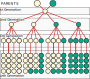
\includegraphics[width=0.95\tfwidth]{figures/mendel-expt.pdf}
\caption{Results of Mendel's experiment with yellow and green peas till fourth generation.\label{mendel-expt}}
\end{figure}

Mendel's results can be seen in \figr{mendel-expt} where the yellow circles are
individuals with the dominant trait, while the green circles are
individuals with the recessive trait. We see a definite pattern. Mendel
discovered this pattern and therefore discovered the mechanism by
which hereditary traits are passed down from generation to generation.
Mendel understood that the pattern had a probabilistic nature.


The pattern of crossings had been observed before Mendel. Suffice it,
for instance, to cite the diary of Mendel's contemporary, a gardener at
the Paris Botanical Gardens: 
\begin{quote}
``Starting from the second generation, the outward appearance changes noticeably. The perfect uniformity of the first generation individuals is usually replaced by an extreme diversity of progeny, some of them being close to the species type of the father and the other close to that of the mother \ldots'' 
\end{quote}
But nobody before Mendel had attempted to investigate the change in separate traits, or count the number of individuals with different traits in consecutive generations. Mendel was the first person to do this, spending eight years on his
experiments. Therefore, unlike his predecessors, Mendel came to
understand the \redem{pattern behind the hereditary transmission of traits}.

It is good to pause here, to discuss the laws governing crossbreeding
which Mendel discovered. We shall do this in the next section from the
viewpoint of modern genetics. Let me only tell the reader that Mendel
presented his results first in February 1865 to the Society of Natural
Scientists in Br\"unn. The audience did not understand the exceptional
importance of the presentation, nor could they guess that it would cause
a revolution in the study of heredity. In 1866, Mendel's paper was published
in the Br\"unn Bulletin and was sent to some 120 listed scientific
institutions in many countries. Unfortunately, Darwin did not receive
a copy.

The world now recognizes Mendel as the founder of modern genetics.
However, the recognition only came in 1900, fifteen years after his
passing.

\section{The Patterns After the Random Combination of Genes in Crossbreeding}

\txthead{Chromosomes and genes.} Perhaps you can recall some data on \redem{cytology}, the branch of biology dealing with the structure, behaviour, growth, and reproduction of cells, and the functions and chemistry of the cell components. There are two types of cell: \redem{germ} cells (\redem{gametes}) and \redem{somatic} cells. The nucleus of each cell contains threadlike structures, \redem{chromosomes}, which carry linearly arranged genetic units in gigantic molecules of deoxyribonucleic acid (DNA) or combination with protein molecules. The chromosomes, or, to be more accurate, the DNA molecules are the carriers of genetic information, which is encoded in the sequence of bases, defining the genotype of the organism. The separate parts of a chromosome, responsible for a hereditary trait, are
the basic units of heredity, or \redem{genes}. Each chromosome contains several hundred genes. Sometimes, a chromosome is viewed as a thread with beads for the genes.

Each species has a fixed \redem{set of chromosomes}. For instance, oats possess 42 chromosomes, \redem{Drosophila} possess 8 chromosomes, chimpanzees possess 48 chromosomes, and human beings have 46 chromosomes. The nucleus of every somatic cell contains all the chromosomes needed for the individual of that species. This means that \redem{each cell} in the organism contains all the individual's \redem{genetic information}.

The numbers of chromosomes we gave for several species characterize
the chromosomes in the somatic cell, rather than in germ cells. Each
germ cell (gamete) has half the number of chromosomes than a somatic
cell.

Let us start with the chromosome set of a somatic cell. This set
includes two \redem{sex chromosomes}. Female individuals have two identical sex
chromosomes (two \redem{X-chromosomes}) while male individuals have two
different sex chromosomes (one \redem{X-chromosome} and one \redem{Y-chromosome}). The somatic chromosomes in a somatic cell come in pairs; the chromosomes in each pair (they are called \redem{homologous}) are very much like each other. Each contains the same number of genes at the same loci on both chromosome threads, and the main point is that they are
responsible for the same kind of trait. For instance, the pea has a pair of
homologous chromosomes each of which contains a gene for seed
colour. This gene, like any other gene, has two forms (they are called
\redem{alleles}), dominant and recessive. The dominant form of the colour gene (the \redem{dominant allele}) corresponds to yellow while the recessive one (the \redem{recessive allele}) corresponds to green. If the genes on both homologous chromosomes contain the same allele, the individual is \redem{homozygotic} with respect to the trait in question. If a chromosome contains an allele which is different from the one contained in the homologous chromosome, the individual is \redem{heterozygotic}. Its phenotype shows the trait corresponding to the dominant allele.

Now let us consider the chromosome set of a gamete (a germ cell).
A gamete has only one sex chromosome. It is always an \redem{X-chromosome} for a female individual. A male individual may contain either an \redem{X-chromosome} (in some gametes) or a \redem{Y-chromosome} (in the other gametes). Besides the single sex chromosome, a gamete contains one chromosome from each pair of homologous chromosomes.


Suppose there are only two pairs of homologous chromosomes, and
a certain trait corresponds to each pair. Moreover, assume the given
individual is heterozygotic with respect to both traits. This individual
will have four types of gamete, which can be seen in \figr{genes0}~\drkgry{(a)} (the red colour in the figure is for the chromosomes with the dominant alleles and the blue colour for the recessive alleles). The individual in \figr{genes0}~\drkgry{(b)} is homozygotic with respect to one trait and heterozygotic with respect to the other. There are only two types of gamete in this case.

\begin{figure}[!ht]
\centering
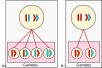
\includegraphics[width=0.9\tfwidth]{figures/genes0.pdf}
\caption{Combination of chromosomes and their results.\label{genes0}}
\end{figure}

During fertilization, a female gamete fuses with a male gamete. The
fertilized egg (called a \redem{zygote}) has a complete chromosome set. Each pair of homologous chromosomes receives one chromosome from the father and one from the mother. The organism develops from a zygote through a series of divisions. The division of the cell is preceded by the \redem{replication} of all the chromosomes contained in the nucleus of the cell. The result is that the nucleus of each somatic cell of the organism contains the same set of chromosomes and genes that the zygote had. When the organism reaches sexual maturity, a special process occurs leading to the production of gametes. We shall discuss this process
below.

\txthead{The law of segregation.} Let us consider one particular trait, for
instance the colour of pea seeds, as in one of Mendel's experiments. Let
us consider the results of this experiment from the point of view of
modern cytology.

All the individuals in the first generation are heterozygotic for the
trait. Each somatic cell contains both alleles for seed colour: yellow
(dominant allele) and green (recessive allele). Naturally, every seed
belonging to these individuals is yellow. Each first-generation individual
has two types of gamete: some with the dominant allele ($A$-gametes) and
the others with the recessive allele ($a$-gametes). It is clear that there must
be both female and male $A$-gametes and $a$-gametes.

Now let us consider the second generation. Each new organism
develops from a zygote which is formed when a male gamete ($A$ or $a$)
fuses with a female gamete ($A$ or $a$). Clearly, four alternatives are
possible (\figr{genes1}):
\begin{mybox}{}
 $AA$ or a male $A$-gamete fuses with a female $A$-gamete,\\
$Aa$ or a male $A$-gamete fuses with a female $a$-gamete,\\
$aA$ or a male $a$-gamete fuses with a female $A$-gamete, and\\
$aa$ or a male $a$-gamete fuses with a female $a$-gamete.
\end{mybox}


\begin{figure}[!ht]
\centering
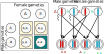
\includegraphics[width=0.9\tfwidth]{figures/genes1.pdf}
\caption{Analysing Mendel's experiment using modern cytology.\label{genes1}}
\end{figure}

\redem{All these alternatives are equally probable.} Therefore, if we take a large enough number of zygotes, a quarter of them will be composed of
$AA$-zygotes, a quarter will contain $aa$-zygotes, and finally, a half will
contain $Aa$-zygotes (the variants $Aa$ and $aA$ are equal from the
viewpoint of trait heredity). If a zygote contains at least one dominant
allele, the phenotype will reveal the dominant feature (yellow seeds).
Therefore, individuals (plants) developing from $AA$- or $Aa$-zygotes will
have yellow seeds while individuals developing from $aa$-zygotes will have
green seeds. We see, therefore, that the probability that \redem{an individual will have a dominant trait is 3/4 while the probability that an individual will
have the recessive trait is 1/4.} Hence the ratio $3:1$ Mendel obtained,
which quantitatively characterizes the segregation of a trait in the
transition from the first generation of the crossing to the second. Mendel
both found this ratio and correctly explained it using the notion of
\redem{probability}. This was \redem{Mendel's first law}, which is also known as the law of segregation.

I want to emphasize: a zygote is formed as the result of the  \redem{random
union} of male and female gametes. A large number of such random
unions will  \redem{necessarily} lead to a definite pattern, which is expressed in the Mendel's first law.

Note that $AA$- and $aa$-zygotes produce homozygotic individuals with
respect to the trait while $Aa$-zygotes produce heterozygotic individuals,
and in the next generation the heterozygotic individuals will produce
a $3:1$ split of traits again.

\txthead{The law of independent assortment of genes.} Suppose we look at the second generation of a crossing involving two traits at the same time.
Let us assume (this is essential) that the genes responsible for the traits
are on different pairs of homologous chromosomes. An example of this
combination is the colour of pea seeds and the shape of the seeds. Let
us use $A$ to denote the dominant allele of colour (yellow), $a$ to denote
the recessive allele of colour (green), $B$ to denote the dominant allele of
shape (smooth seeds), and $b$ to denote the recessive allele of shape
(wrinkled seeds).

\begin{figure}[!ht]
\centering
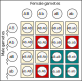
\includegraphics[width=0.75\tfwidth]{figures/genes2.pdf}
\caption{Analysing Mendel's experiment using modern cytology.\label{genes2}}
\end{figure}


Each first-generation individual has four types of male and four types
of female gamete: $AB, \,\, Ab,\,\, aB$, and $ab$ (recall \figr{genes0}~\drkgry{(a)}). A zygote is formed when two gametes (male and female) of any of the four types fuse. There are 16 possible alternatives; they are presented in \figr{genes2}. \redem{Each alternative is equally probable.} Therefore, the ratio of the number of zygotes of different types (with respect to the total number of zygotes, which should be large) is: \vspace{-15pt}
\begin{center}
\begin{tabular}{l}
1/16 for zygotes $AB \cdot AB$, \\
1/16 for $Ab \cdot Ab$, \\
1/16 for $aB \cdot aB$, \\
1/16 for $ab \cdot ab$, \\
1/8 for $AB \cdot Ab$ (including $Ab \cdot AB$, \\
1/8 for $AB \cdot aB$ (including $aB \cdot AB$),\\
1/8 for $AB \cdot ab$ (including $ab \cdot AB$), \\
1/8 for $Ab \cdot aB$ (including $aB \cdot Ab$), \\
1/8 for $Ab \cdot ab$ (including $ab \cdot Ab$), and \\
1/8 for $aB \cdot ab$ (including $ab \cdot aB$). 
\end{tabular}
\end{center}
\vspace{-15pt}

Regarding the suppression of recessive alleles by the corresponding dominant alleles,
we can conclude that the probability that an individual will have yellow
smooth seeds in the second generation equals the sum of probabilities
for the zygotes $AB\cdot AB, \,\, AB \cdot Ab,\,\, AB \cdot aB, \,\, Ab \cdot ab,$ and $Ab\cdot ab$, i.e. $1/16 +
1/8 + 1/8+ 1/8 + 1/8 = 9/16$. The probability that an individual will have
yellow wrinkled seeds equals the sum of probabilities of the formation of
zygotes $Ab \cdot  Ab$ and $Ab \cdot  ab$, i. e. $1/16 + 1/8 = 3/16.$ The probability that
an individual will have green smooth seeds equals the sum of
probabilities of the formation of zygotes $aB \cdot  aB$ and $aB \cdot  ab$, i.e. $1/16 + 1/8 = 3/16$. And finally, the probability that an individual will have
green wrinkled seeds equals the probability of the formation of the
zygote $ab \cdot  ab$, i. e. 1/16. Therefore, the numbers of different phenotypes (with these traits) in the second generation are in the ratio $9 :3 : 3 : 1$. This is the essence of \redem{Mendel's second law}, according to which the segregation by one trait is \redem{independent} from the segregation by another
trait.


\txthead{Morgan's Law.} The law of the independent assortment of genes is valid when the genes are on different chromosomes in a gamete (and on
different pairs of homologous chromosomes iii a somatic cell). If the
genes belong to the \redem{same} chromosome, they will be inherited together. This is the explanation for deviations from Mendel's second law. The deviation was discovered and investigated by the American biologist
Morgan and is observed whenever traits are defined by linked genes, i.e.
the genes are on the same chromosome. The joint inheritance of linked
genes became known as \redem{Morgan's law}.

Thomas Hunt Morgan (1866-1945) was the founder of the
chromosome theory of inheritance. By introducing the idea of
a chromosome, he substantiated Mendel's laws and pointed out under
which conditions they are applicable. Besides, he obtained a number of
new results. These results include Morgan's law and the phenomenon of
chromosome crossing over, which he discovered.

\txthead{Chromosome crossing over.} In an investigation of the inheritance of traits defined by linked genes, Morgan discovered that the linkage \redem{is not absolute}: some of the second-generation individuals inherit some of the linked genes from one parent and the rest from the other. Carrying out
his investigations on \redem{Drosophila}, Morgan could explain this fact. He
showed that the formation of germ cells in an organism (this process is
called \redem{meiosis}) starts with a ``farewell dance'' of homologous
chromosomes. 

Imagine two elongated homologous chromosome threads, which,
before they leave each other and join different gametes, tightly embrace
each other (each gene in contact with the corresponding gene) and then
wind around each other several times. This winding of the chromosomes
(crossing over) results in the intracellular forces which arise to pull the
chromosomes apart, \redem{break} them. The site where the break occurs varies randomly from one pair of crossed-over chromosomes to another. The result is that one gamete receives \redem{complementing} parts of both homologous chromosomes rather than an intact chromosome, and the other parts of these chromosomes are received by the other gamete. The process is illustrated in \figr{genes3}. Let me emphasize that corresponding genes on both chromosomes (I mean the alleles) are in contact with each other at the moment of break. Therefore, wherever the break might be, an allele from one chromosome gets into one gamete while an allele from the other chromosome gets into the other gamete. In other words, either gamete gets an allele with the considered gene. This can be thought of as ``dancing'' pairs of chromosomes exchanging equivalent parts of themselves before leaving each other. All the same, each gamete has a complete set of genes characterizing the given chromosome. And there is a \redem{random combination} of paternal and maternal alleles.

\begin{figure}[!ht]
\centering
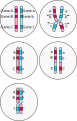
\includegraphics[width=0.7\tfwidth]{figures/genes3.pdf}
\caption{``Farewell dance'' of the genes combines genes from the two parents.
\label{genes3}}
\end{figure}


Chance plays an essential role in the phenomenon of chromosome
crossing over. The site of the break is \redem{random} in a pair of chromosomes, and therefore, the combination of parental alleles is  \redem{random}.

By expanding the domain of the random, the phenomenon of
chromosome crossing over enhances intra-species development, creating
additional possibilities for ``shuffling'' the parental genes. At the same
time, the phenomenon, as it were, protects the species from random
genetic ``infringements''. Suppose individuals from two different species
cross at random and hybrids appear. Each ``homologous pair'' in the
hybrids unites chromosomes that are very unlike in their gene structure
(because the chromosomes come from parents of different species). When
the time comes to produce the germ cells, these chromosomes are
unable to carry out the ``farewell dance'' because of fundamental
differences. They consequently are unable to form gametes, and therefore,
no second-generation hybrids appear. This is why mules (the
hybrid offspring of a male ass and a female horse) do not have any
progeny.

\txthead{A boy or a girl?} I have already noted that the sex chromosomes of
a female are both the same: they are $X$-chromosomes. By contrast, the
sex chromosomes of a male are different, each male having one
$X$-chromosome and one $Y$-chromosome. Half of all male gametes carry
one $X$-chromosome and the rest carry one $Y$-chromosome. If a female
gamete joins a male $X$-gamete, an $XX$-zygote is produced, and a female
offspring develops from it. But if a female gamete fuses with a male
$Y$-gamete, an $XY$-zygote is produced, and a male offspring develops from it. This is the answer to the question: a boy or a girl?

\section{Mutations }%
We have considered random changes in the genetic code that might
occur when a combination of parental genes is crossed over. All these
changes are limited by the available gene pool. New genes cannot be
created in the process. However, random inheritable changes do occur
which are not related to the combination of genes. They are caused by
the action of the environment on the genetic structure of the
chromosomes and random disorders in the biological mechanism that
maintains the genetic information during meiosis and the division of the
somatic cells. These genetic changes are called \redem{mutations}.

\txthead{The appearance of mutations.} There is a serious human disease in
which a sufferer's blood is unable to clot. This disease is called \redem{hemophilia}. It is inherited and occurs in men only. It has been found out that hemophilia is the consequence of a \redem{mutation} in a gene that is located on the $X$-chromosome. Since women have two $X$-chromosomes, the mutated gene, which is recessive, on one chromosome is matched by
a normal gene on the other, which suppresses the illness. This is why
women do not suffer from hemophilia. This is not the case in men. The
set of sex chromosomes in men consists of two \redem{different} chromosomes: one $X$-chromosome and one $Y$-chromosome. There is no normal paired gene which can suppress the hemophilia gene. Consequently a man receiving an $X$-chromosome with the mutated gene from a phenotypically healthy mother suffers from hemophilia.

Fortunately, mutations are mostly harmless. A short-fingered hand,
a sixth finger, and the heart on the right are relatively rare mutations.
More frequent mutations show themselves as, for instance, different eye
colours, baldness (including the shape of the bald spot), and unusual
hair colour in animals. Mutations often occur in plants and appear in
a great variety of ways, such as changes in the shape of the stem, leaves,
and flowers.

\txthead{The causes of mutations.} A mutation is a rather rare event. For
instance, the probability that a gamete with an $X$-chromosome taken at
random will contain the mutation related to hemophilia is only one in
\num{d5}. Other mutations occur even less often, with the probability of about one in \num{d6} on the average. However, we should take into account the diversity of mutations. They can be associated with very different genes
of which there is an enormous number in each gamete. We should also
take into account that mutations are inherited and thus \redem{accumulate}. The
result is that mutations per se are not too rare events. It has been
calculated that one in ten human gametes carries a mutation.

The appearance of each mutation is a \redem{random} event. However, the
event results from objective causes. An organism develops from a zygote
due to the cell divisions. The process of cell division begins with
replication of chromosomes, and therefore, DNA molecules in the cell
nucleus. Each DNA molecule recreates an exact copy of itself with the
same set of genes. The complicated process of replication of a DNA
molecule sometimes occurs with random deviations. We know that
genetic information is recorded in DNA very economically on the
molecular level. When the data is copied, various kinds of ``misprint'' are
possible due to the thermal movement of molecules. The ``misprints''
appear due to the unavoidable \redem{fluctuations} in the behaviour of matter. For instance, when a DNA molecule replicates, there might be
a random increase in the number of hydrogen ions in the vicinity of
some nitrogen base. This fluctuation may cause the detachment of the
base from the DNA, i.e. to a disturbance in the structure of the gene.

In every sexually reproducing species, the progeny only receive the
mutations in the germ cells. Therefore, the random disordering that
occurs in the formation of the germ cells, in meiosis, is essential. These
disorders may cover both separate genes and chromosomes as a whole.
Individual gametes may receive a chromosome with a distorted gene
structure or not receive a chromosome at all. The formation of gametes
with extra chromosomes is also possible.


The thermal movement of matter molecules is not the only cause of
mutation. Special investigations have revealed a number of \redem{external}
factors which cause mutations .and are called \redem{mutagenic} factors. Certain
chemicals and various kinds of radiation, e. g. $X$-rays, neutron beams,
fast charged particles, are all mutagenic.


\txthead{Advantages and disadvantages of mutations.} From the viewpoint of
evolution, mutations are certainly advantageous. Moreover, they are
necessary. The vast diversity of genes in each species and the diversity of
species existing on the Earth are a consequence of mutations having
occurred over many millions of years, and they still occur. From the
point of view of an individual, as a rule, mutations are harmful and even
lethal more often than not. Being the result of long-term evolution, each
organism is a complex genotype and adapted to its habitat. A random
change in the genotype would more likely disrupt its smoothly running
biological mechanism.

Therefore, we see that mutations are at the same time both useful
(even necessary) and harmful. If mutations occur too frequently in
a given species (for instance, because its habitat is radioactively
contaminated), this will increase the mortality rate and, as
a consequence, cause the decline or possibly the extinction of the
species. By contrast, if mutations occur too rarely in a given species, it
may not be able to adapt and may also become extinct should its
habitat change considerably. For instance, the dinosaurs could not
adapt to a cooling in the climate and became extinct. Thus, it is
disadvantageous for there to be too many mutations or for them to be
too frequent. It is also disadvantageous for there to be practically no
mutations or for them to occur too rarely.

\txthead{The Organism and mutations.} The adaptation of an organism to its
habitat also supposes the adaptation to mutations, owing to which the
degree of harm brought about by mutations can be essentially reduced.
This adaptation is natural because the development of species is directly
related to its survivability.

Let us discuss this problem from the positions of genetics. Suppose
a zygote appears when a normal and a mutated gamete combine. We
shall call a gamete mutated if one of its chromosomes has a faulty
(mutated) gene. Suppose this gene is responsible for a vital process, and
so we are dealing with a dangerous mutation. The mutated gene is
opposed by the normal gene in the paired chromosome. Now mutated
gene may either be dominant or recessive with respect to the normal
gene, and we shall consider both possibilities.

If the mutated gene is \redem{dominant}, it immediately starts its ``harmful
activity'', and the organism may die as an embryo. Darwinian selection
here carries out its sanitary mission long before the dominant mutation
can propagate to future progeny. The result is that there is no accumulation
of dominant mutated genes. This is not so if the mutated gene
is \redem{recessive}. It is suppressed by the normal gene, and therefore, the
organism will be phenotypically healthy. Moreover, there will be healthy
organism phenotypes in the progeny. It is only in rare cases that the
recessive mutated gene reveals itself, i.e. when a descendant gets the
gene simultaneously through the paternal and maternal gametes.

I would very much like to say that the Nature has taken care to
decrease the danger of harmful mutations. However, recall that the
Nature never takes care of anything or anybody. The principle is the
selection of the fittest. There is no ``wisdom'' in the Nature.

Unfortunately, people sometimes increase the danger of mutations.
The probability that two recessive genes will combine in a descendant
increases if close relatives marry or a \redem{small group} of people, for instance, a small religious sect, small community, or the population of a hamlet in the mountains, intermarry. Wherever this practice is common, various types of genetic disease are unavoidable (they are called \redem{recessive diseases}). There are about five hundred such diseases known so far. They may bring about idiocy, debility, deaf-mutism, constitutional inferiority, etc. Therefore, any artificial separation or division of people into closed groups increases the genetic danger and leads to a higher probability of recessive disease.

In the second half of this century, the mutation danger drastically
increased due to nuclear weapon testing. Radioactivity is very mutagenic.
Therefore, it is impossible to overestimate the importance of the
international treaty banning the testing of nuclear weapons in the
atmosphere, space, and underwater, which was concluded at the
initiative of the Soviet Union. In 1963, the treaty was signed by the
USSR, USA, and Great Britain. Over a hundred countries have signed it
so far.

\txthead{The law of homologous series in hereditary variability.} Each
individual mutation is a random, undirected, and unpredictable event. If
a given species sustains relatively many mutations (this is seen in plants),
the picture of mutations on the whole shows some \redem{regularity}, or
necessity. This is substantiated by the \redem{law of homologous series} in
mutations discovered by the Soviet biologist Nikolai I. Vavilov
(1887-1943). Generalizing a great deal of data, Vavilov concluded that
genetically close species should be characterized by similar (homologous)
series of hereditary variability. For instance, if mutations cause
a number of rather frequently occurring hereditary traits in rye,
a similar series of traits should also be observed in wheat, barley, oats,
etc.

Vavilov's law is sometimes compared to Mendeleev's periodic table,
thus emphasizing that like the periodic table it can be used to predict
new members, or mutants. In 1917, during a scientific expedition in the
Pamir, Vavilov found a variety of wheat with leaves without a ligule,
a small growth at the base. At the time, biologists were not aware of rye
or barley varieties without ligules. However, Vavilov's law required that
they exist, and in 1918 a variety of rye was found without ligules, while
in 1935, a barley variety without ligules was obtained after irradiating
common barley with X-rays.

\section{Evolution Through the Eyes of Geneticists}

There was a time when some biologists tried to oppose the theories of
Darwin and Mendel. This should be regarded as a frustrating mistake
and seems absurd today. It is generally recognized that genetics have
put Darwin's theory of the origin and evolution of species on a sound scientific basis, and explained the hereditability of changed traits. Darwinism is a logical and authoritative science capable of giving valuable practical recommendations. Modern genetics is deeply rooted in Darwinism.


\txthead{Undirected hereditary variability.} The Soviet biologist Ivan Shmalgausen (1884-1963) once said that each species and each of its populations contain a ``pool of hereditary variability''. This pool can be utilized by natural selection in a changed habitat.


There are two basic ``mechanisms'' for the appearance of undirected hereditary variability. Firstly, there is \redem{mutation variability}. Mutations underlie the diversity of species and the diversity of genes within a species. Mutation changes occur very slowly, but they occur continuously and have done so since the time immemorial. The ``mechanism'' by which hereditary variability appears as the result of the random crossing of \redem{parental} genes is faster. Here we should distinguish between the combination of genes as the result of fusing random pairs of gametes and the combination of genes as the result of ``shuffled'' parts of paired chromosomes getting randomly into a gamete (the phenomenon of chromosome crossing over).


Naturally, the changes in the combination of genes are limited by the volume of the gene pool. However, the pool is enormous. It has been calculated that the gene pools of a father and a mother make it possible in principle to construct up to \num{d50} different human genotypes. This is a rather hard number to imagine. Less than \num{d10} people live on the Earth. Therefore, there is practically no chance that two individuals will be genetically identical (unless, of course, they are twins developing from the same zygote). Each person is \redem{genetically} unique; a person possesses a genotype which is unlike any other genotype.


\txthead{Darwin's demon versus Maxwell's demon.} We discussed the Maxwell's demon in Chapter~4. Without getting outside information, the demon could not in principle select faster molecules and direct them into the other half of the vessel. This hapless demon demonstrated the fundamental \redem{impossibility of selection at the atomic or molecular level}, as was demanded by the second law of thermodynamics.


In a discussion on natural selection in the Nature, the American biochemist and science-fiction writer Isaac Asimov (1920-1992) used the term ``Darwin's demon''. Unlike Maxwell's hapless demon, Darwin's demon operates very successfully, selecting organisms with a better
chance for survival and letting them reproduce and move into the next
generation. The major distinction between the Darwin's and Maxwell's
demons is that they operate on \redem{different} levels. Anything begins at the atomic or molecular level. Random, undirected mutation and the
random combinations of genes occur at this level. If Maxwell's demon
could operate, he would start by selecting the most ``advantageous''
mutations and the most ``successful'' combinations of genes. This does not occur because selection is impossible at atomic or molecular level. 



And here is where the \redem{principle of reinforcement} starts. Suppose that a mutated gene has got into a zygote. While the organism develops, the cells divide, and the result is that the mutated gene is replicated about
\num{d15} times. The combination of genes in the zygote has also been replicated. Therefore, \redem{random changes} in the genetic code in the process of the development of the phenotype becomes \redem{reinforced}. And this is a transition from the atomic or molecular level to the level of \redem{macrophenomena}. Selection at this level is possible. I want to emphasize: Darwin's demon does not try to select different genetic codes, and in this sense it is not quite like Maxwell's demon. It influences the organism's phenotypes, where any change in the genetic code is amplified about \num{d15} times.


There should be no need to explain how Darwin's demon operates. The way natural selection is realized is described in every textbook on biology. Let me only note that the ``demon'' is rather merciless. It operates severely: it eliminates phenotypes which have randomly proved unfit. Taking those which are randomly less or more fit to the habitat, it gives preference to the more fit while the less fit are, as a rule, eliminated.


However, Darwin's demon does not operate directly and gives the less fit a chance to survive. Changes in the genetic code which may not be used today may be utilized tomorrow. They are useless and even harmful today, but they may become useful later. It means that we should not hurry and render the verdict. Let the random variation in the genetic code ``sleep'', stay dormant for a while, for several generations of phenotypes, masked as a recessive gene. It may suddenly be helpful later.


Naturally, the effect of Darwin's demon or, in other words, natural selection does not oppose the second law of thermodynamics in any way. We noted above, that living beings only exist due to the inflow of negentropy from the environment, i.e. due to the rise of entropy in this environment. This increase in entropy is the ``fee'' for the service provided by Darwin's demon.


\txthead{Diversity of species.} The diversity of species on the Earth, where
\redem{Protozoa} coexist with very complicated and organized species, is the
result of evolution proceeding for about two thousand million years. 
Two thousand million years ago the Earth was only inhabited by
bacteria and blue-green algae. Several hundred million years later,
unicellular organisms with a cellular nucleus appeared. After a period of
several hundred million years more, \redem{Coelenterata}, worms, and molluscs appeared. About five hundred million years ago, fish appeared, followed by amphibia, and still later by reptiles. Mammals appeared about
a hundred million years ago. Note that there is no mere transition from
less complicated species to more complicated ones in this evolutionary
process. Naturally, many species became extinct; nevertheless, today
a tremendous number of simple species exist alongside complicated
ones. Evolution has been directed \redem{from the less fit to the more fit} rather than \redem{from the simple to the complicated} because natural selection
operates in this direction and no other one. The characteristic feature of
this process is the \redem{increase in the number of species} and their growing diversity. Higher species will appear, which is an advance for the
evolution process.

We could give a number of reasons why evolution increases the
number of species. Firstly, hereditary variability increases in time, i.e.
mutations accumulate and the gene pool extends. Secondly, there are
a great number of ways to adapt to any given change in the
environment. Natural selection approves of any acceptable versions. The
selected variants may have either a more or less complicated
organization. Thirdly, once it has appeared, a species has a certain
stability. In particular, it resists the danger of being incorporated by
other species. Recall that hybrids produced by crossing between different
species cannot form germ cells, and therefore, cannot have any progeny.
Naturally, when we consider the increase in the number of species, we
have to take into account the reverse processes, such as the elimination
of a species due to an interspecific struggle or the extinction of a species
because of its inability to adapt to sudden severe changes in the
environment.

\txthead{Unpredictability of new species.} We considered fluctuations in an
ensemble of gas molecules in Chapter~4 and saw how the fluctuations of
the variables for an individual molecule are great. They are comparable
to the means of the variables. On the contrary, fluctuations of the
variables for a macrosystem are extremely small. Therefore,
a macro system could be described on the basis of dynamic laws rather
than probabilistic laws. This is done in thermodynamics. This means
that the transition from the atomic or molecular level of consideration
to the macrolevel brings about, as it were, a reciprocal compensation of
numerous random deviations in the behaviour of individual molecules.
The result is that the behaviour of the macrosystem as a whole becomes
unpredictable unambiguously.

As to Nature, we encounter a qualitatively different situation. The
individual fluctuations characterizing random changes in the genetic
code are reinforced \num{d15} times and can be revealed on the macro level, in the organism phenotype. There is no reciprocal compensation here. \redem{Each fluctuation grows to macroscopic dimensions.} Therefore, we can assert that the process of evolution in the Nature is \redem{fundamentally unpredictable} in the sense that no one can foresee the emergence of concrete species. In other words, each species proves to be a random phenomenon. It can be eliminated, a new species can be created, but an extinct species cannot be restored. Each existing species is unique in this sense.

\txthead{Conclusion} We have discussed a number of problems in biology
related to genetics and evolution theory. These problems clearly show
the \redem{fundamentality of probabilistic laws} and the \redem{fundamental role of chance}. However, the topic of probability in biology is much wider. It
also includes a number of problems that could not be treated in this
book, such as the origin of life on the Earth, the change in the sizes of
populations of species, the simulation of the nervous system, and the
creation of a model of the human brain.
%%% Local Variables:
%%% mode: latex
%%% TeX-engine: xetex
%%% TeX-master: "twibop2"
%%% End:
